\section{Цель работы}

\begin{enumerate}
    \item Провести измерения направления суммарного магнитного поля, создаваемого Землей и системой катушек Гельмгольца.
    \item Определить горизонтальную составляющую магнитного поля Земли.
\end{enumerate}

\section{Объект исследования}

Магнитное поле Земли; система катушек (колец) Гельмгольца.

\section{Метод эксперимента}

В данной работе используется метод суперпозиции магнитных полей. На магнитную стрелку компаса, помещенную в центре колец Гельмгольца, одновременно действуют горизонтальная составляющая магнитного поля Земли $\vec{B}_h$ и магнитное поле катушек $\vec{B}_c$, направленное под углом $\varphi$ к $\vec{B}_h$. Измеряя угол отклонения $\alpha$ стрелки от исходного положения при различных значениях тока в катушках, можно определить величину $B_h$ путем линейной аппроксимации зависимости $B_c(\gamma)$, где $\gamma = \sin\alpha / \sin(\varphi - \alpha)$.

\section{Измерительные приборы}

\begin{table}[h]
\centering
\begin{tabular}{|c|c|c|c|}
\hline
№ & Наименование & Используемый диапазон & Погрешность \\
\hline
1 & Амперметр & 0-50 мА & 0.1 мА \\
\hline
2 & Транспортир & 0-160° & 0.5° \\
\hline
\end{tabular}
\end{table}

\section{Схема установки}

\begin{figure}[h]
    \centering
    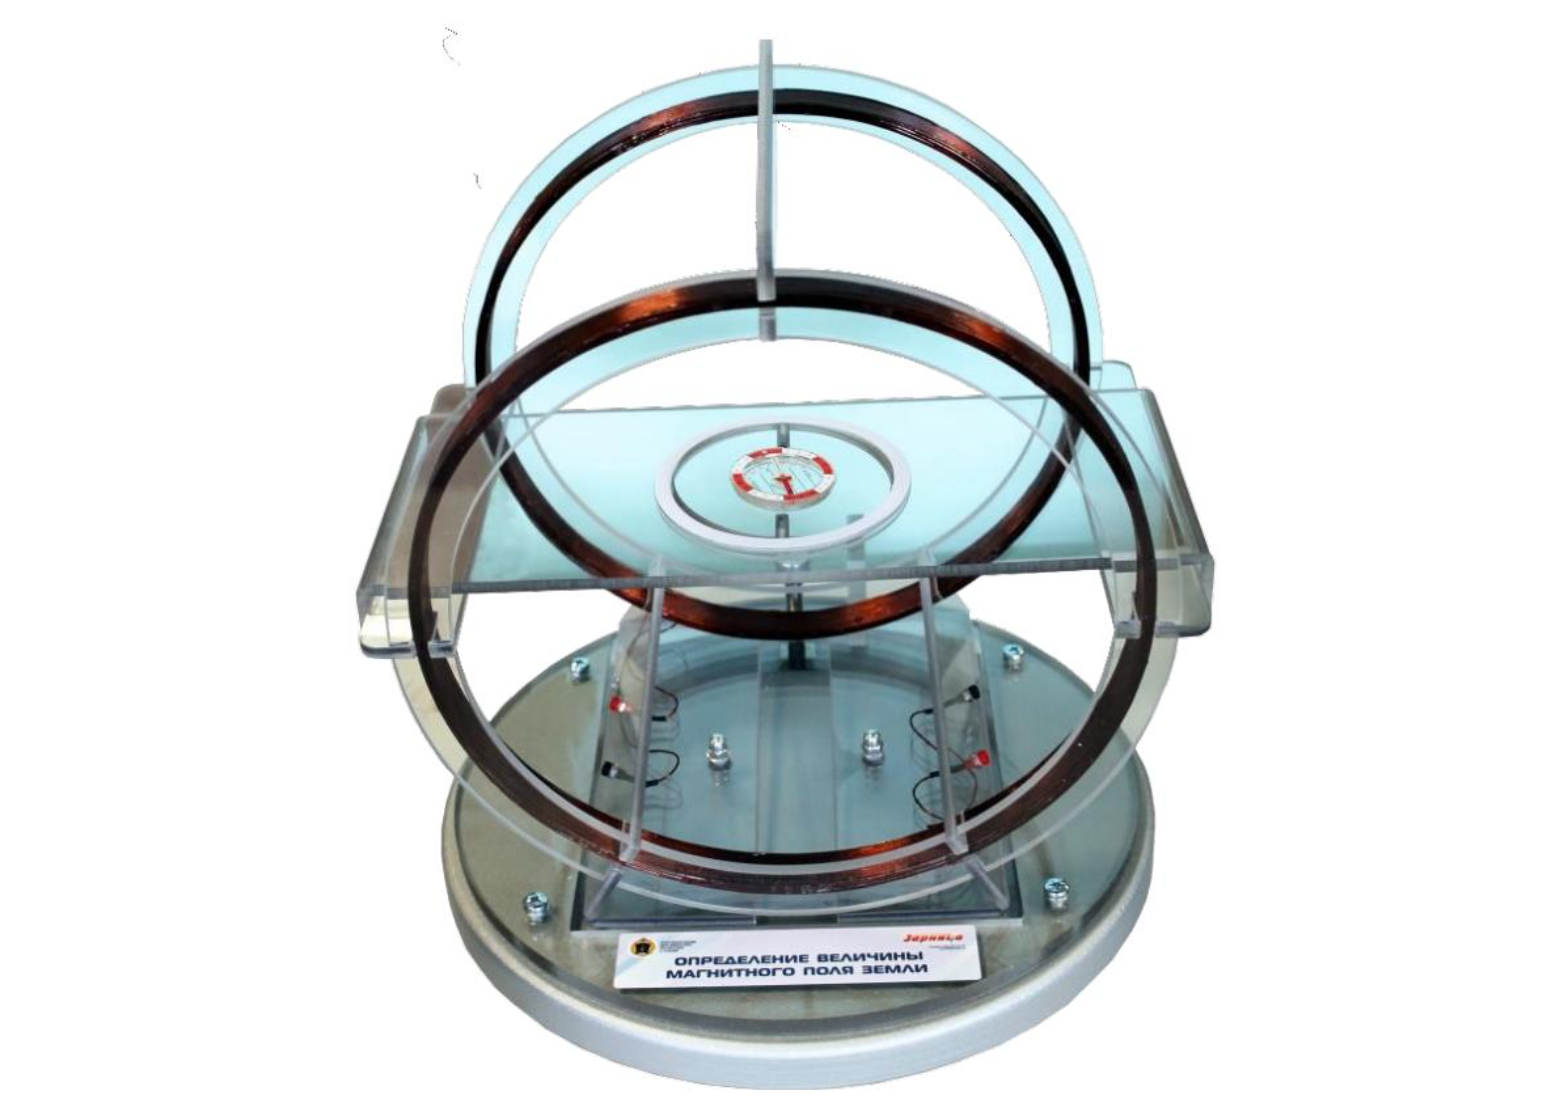
\includegraphics[width=0.65\linewidth]{pic/1780093326735.png}
    \caption{Лабораторная установка: кольца Гельмгольца с компасом в центре}
    \label{fig:scheme}
\end{figure}

Лабораторная установка включает в себя последовательно соединенные кольца Гельмгольца с компасом в центральной части, источник питания со встроенным амперметром и токоограничивающее сопротивление. Кольца Гельмгольца смонтированы на устойчивом основании и расположены параллельно друг другу.

\section{Рабочие формулы и исходные данные}

\subsection{Исходные данные}

\begin{center}
\begin{tabular}{|l|c|l|}
\hline
\textbf{Параметр} & \textbf{Обозначение} & \textbf{Значение} \\
\hline
Радиус катушек & $R$ & $0{,}15$~м \\
\hline
Число витков в каждой катушке & $n$ & $100$ \\
\hline
Угол между осями катушек и магнитным меридианом & $\varphi$ & $160^\circ$ \\
\hline
Магнитная постоянная & $\mu_0$ & $4\pi \cdot 10^{-7}$~Гн/м \\
\hline
\end{tabular}
\end{center}

\subsection{Рабочие формулы}

Магнитная индукция поля катушек Гельмгольца в центре системы:

\begin{equation}
B_c = \mu_0 \left(\frac{4}{5}\right)^{3/2} \frac{I n}{R}.
\label{eq:Bc}
\end{equation}

Из теоремы синусов для треугольника, образованного векторами $\vec{B}_h$, $\vec{B}_c$ и результирующего поля (рис. 5 описания), следует:

\begin{equation}
\frac{\sin\alpha}{\sin(\varphi - \alpha)} = \frac{B_c}{B_h}.
\label{eq:sine}
\end{equation}

Введём обозначение:

\begin{equation}
\gamma = \frac{\sin\alpha}{\sin(\varphi - \alpha)}.
\label{eq:gamma}
\end{equation}

Тогда:

\begin{equation}
B_c = B_h \cdot \gamma.
\label{eq:linear}
\end{equation}

Таким образом, построив график зависимости $B_c(\gamma)$ по экспериментальным точкам и определив его угловой коэффициент методом наименьших квадратов (МНК), находим горизонтальную составляющую индукции магнитного поля Земли $B_h$.

\section{Результаты измерений и обработки}

\subsection{Таблица прямых и косвенных измерений}

Угол $\varphi = 160^\circ$ установлен при ориентировании основания колец. Для каждого значения угла отклонения $\alpha_i$ проведено по три измерения тока $I_1, I_2, I_3$. По формуле (\ref{eq:Bc}) вычислено поле катушек $B_c$:

\[
B_c = \mu_0 \left(\frac{4}{5}\right)^{3/2} \frac{\langle I \rangle n}{R}
    = 4\pi \cdot 10^{-7} \cdot 0{,}71554 \cdot \frac{\langle I \rangle \cdot 100}{0{,}15}
    \approx 5{,}9945 \cdot 10^{-4} \cdot \langle I \rangle \text{ (Тл)}
    = 0{,}5995 \cdot \langle I \rangle \text{ (мкТл, если $\langle I \rangle$ в мА)}.
\]

\textbf{Пример расчета} (для $\alpha = 10^\circ$):
\[
\langle I \rangle = (11 + 12 + 14) / 3 = 12{,}33 \text{ мА},
\]
\[
B_c = 0{,}5995 \cdot 12{,}33 = 7{,}39 \text{ мкТл},
\]
\[
\gamma = \frac{\sin 10^\circ}{\sin(160^\circ - 10^\circ)} = \frac{0{,}1736}{0{,}5000} = 0{,}3473.
\]

Результаты всех вычислений сведены в таблицу~1.

\begin{table}[H]
\centering
\caption{Результаты измерений и вычислений ($\varphi = 160^\circ$)}
\small
\begin{tabular}{|c|c|c|c|c|c|c|}
\hline
$\alpha_i$ & $I_1$, мА & $I_2$, мА & $I_3$, мА & $\langle I \rangle$, мА & $\gamma_i$ & $B_c$, мкТл \\
\hline
$10^\circ$  & 11 & 12 & 14 & 12{,}33 & 0{,}3473 & 7{,}39 \\
$20^\circ$  & 20 & 18 & 20 & 19{,}33 & 0{,}5321 & 11{,}59 \\
$30^\circ$  & 23 & 23 & 21 & 22{,}33 & 0{,}6527 & 13{,}39 \\
$40^\circ$  & 26 & 25 & 26 & 25{,}67 & 0{,}7422 & 15{,}39 \\
$50^\circ$  & 31 & 31 & 31 & 31{,}00 & 0{,}8152 & 18{,}58 \\
$60^\circ$  & 34 & 34 & 34 & 34{,}00 & 0{,}8794 & 20{,}38 \\
$70^\circ$  & 35 & 36 & 35 & 35{,}33 & 0{,}9397 & 21{,}18 \\
$80^\circ$  & 39 & 38 & 37 & 38{,}00 & 1{,}0000 & 22{,}78 \\
$90^\circ$  & 41 & 40 & 40 & 40{,}33 & 1{,}0642 & 24{,}18 \\
$100^\circ$ & 42 & 43 & 43 & 42{,}67 & 1{,}1372 & 25{,}58 \\
$110^\circ$ & 47 & 45 & 45 & 45{,}67 & 1{,}2267 & 27{,}37 \\
$120^\circ$ & 50 & 49 & 49 & 49{,}33 & 1{,}3473 & 29{,}57 \\
$130^\circ$ & 56 & 56 & 55 & 55{,}67 & 1{,}5321 & 33{,}37 \\
$140^\circ$ & 72 & 68 & 70 & 70{,}00 & 1{,}8794 & 41{,}96 \\
\hline
\end{tabular}
\normalsize
\end{table}

\subsection{Определение $B_h$ методом МНК}

По данным таблицы~1 построен график зависимости $B_c(\gamma)$ (рис.~\ref{fig:Bc_gamma}). Согласно формуле (\ref{eq:linear}), зависимость должна быть линейной и проходить через начало координат. Проведена линейная аппроксимация методом наименьших квадратов:

\[
B_c = k \cdot \gamma + b.
\]

Результаты МНК:
\[
k = 22{,}49 \text{ мкТл}, \qquad \sigma_k = 0{,}43 \text{ мкТл},
\]
\[
b = -0{,}31 \text{ мкТл}, \qquad \sigma_b = 0{,}47 \text{ мкТл}.
\]

Свободный член $b$ отличен от нуля на $0{,}7\sigma_b$, что статистически незначимо. Это подтверждает корректность модели $B_c = B_h \cdot \gamma$ (отсутствие систематического смещения).

Угловой коэффициент графика равен искомой величине горизонтальной составляющей магнитного поля Земли:

\[
\boxed{B_h = 22{,}5 \pm 0{,}4 \text{ мкТл}}.
\]

Относительная погрешность: $\varepsilon = 0{,}4 / 22{,}5 \approx 1{,}8\%$.

\subsection{Сравнение с табличным значением}

Согласно Международной модели главного магнитного поля Земли (IGRF-14, эпоха 2026~г.), для Санкт-Петербурга ($\varphi \approx 60^\circ$ с.ш., $\lambda \approx 30^\circ$ в.д.) горизонтальная составляющая индукции магнитного поля составляет:

\[
B_h^\text{(табл)} \approx 14{,}8 \text{ мкТл}.
\]

Отклонение экспериментального значения от табличного:
\[
\delta = \frac{|22{,}5 - 14{,}8|}{14{,}8} \cdot 100\% \approx 52{,}02\%.
\]

Возможные причины расхождения:
\begin{enumerate}
    \item Наличие ферромагнитных элементов в строительных конструкциях здания (железобетонная арматура, стальные балки), искажающих локальное магнитное поле.
    \item Близость лабораторного оборудования и электропроводки, создающих паразитные магнитные поля.
    \item Неточность установки угла $\varphi = 160^\circ$ и погрешность визуального отсчета угла отклонения стрелки компаса ($\pm 1^\circ$).
    \item Трение в опоре магнитной стрелки, приводящее к занижению угла отклонения $\alpha$ и, как следствие, к систематическому завышению определяемого $B_h$.
    \item Неполная однородность поля катушек Гельмгольца в области расположения компаса.
\end{enumerate}

\section{График}

\begin{figure}[H]
    \centering
    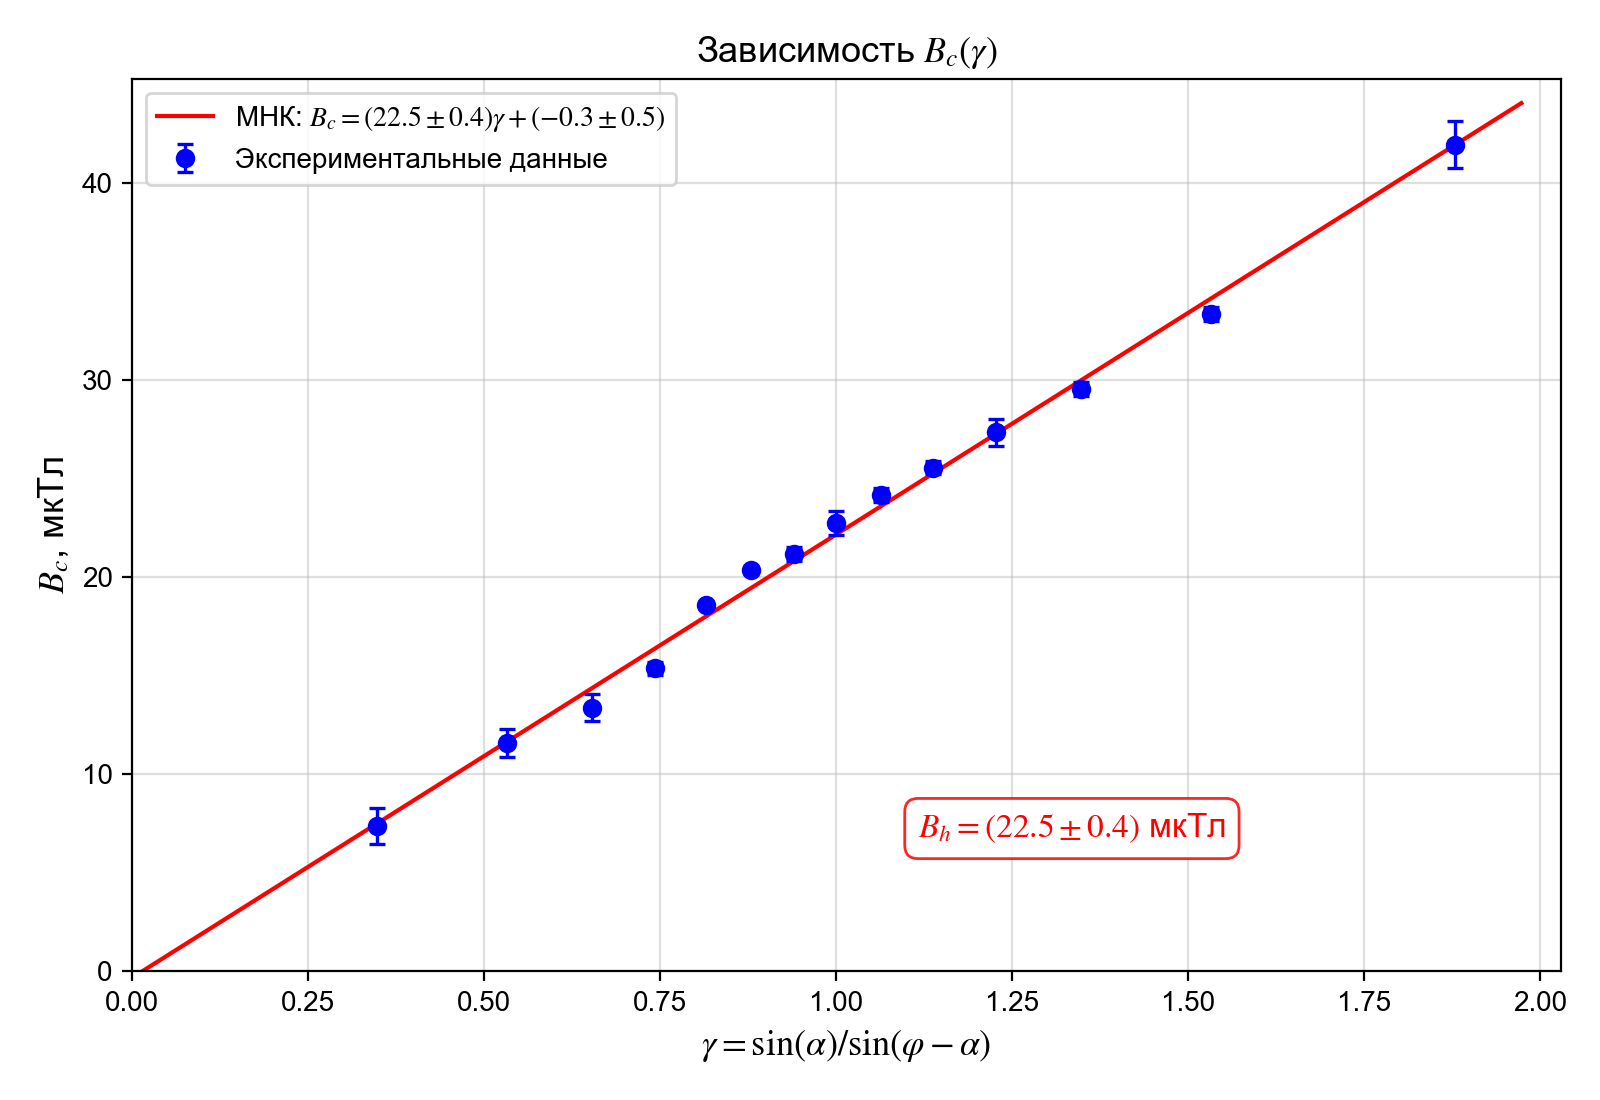
\includegraphics[width=0.85\linewidth]{pic/Bc_vs_gamma.png}
    \caption{Зависимость $B_c(\gamma)$ и линейная аппроксимация МНК}
    \label{fig:Bc_gamma}
\end{figure}

\section{Вывод}

В ходе работы исследовано магнитное поле Земли методом суперпозиции с пробным полем катушек Гельмгольца. Проведены измерения угла отклонения магнитной стрелки компаса при различных токах в катушках в диапазоне $\alpha = 10^\circ \div 140^\circ$. Для каждого значения $\alpha_i$ выполнено по три измерения тока, рассчитаны средние значения $\langle I \rangle$, величины индукции поля катушек $B_c$ и параметра $\gamma = \sin\alpha / \sin(\varphi - \alpha)$.

Построен график зависимости $B_c(\gamma)$, имеющий линейный характер в соответствии с теоретической моделью. Методом наименьших квадратов определена горизонтальная составляющая индукции магнитного поля Земли:

\[
B_h = (22{,}5 \pm 0{,}4) \text{ мкТл}.
\]

Полученное значение превышает табличное ($\sim 14{,}8$~мкТл для региона Санкт-Петербурга) примерно на $52{,}02\%$. Основными причинами расхождения являются локальные искажения магнитного поля ферромагнитными элементами конструкции здания и трение в опоре компаса. В условиях специализированной магнитометрической лаборатории с компенсацией магнитных помех точность метода может быть существенно выше.

Тем не менее, линейный характер зависимости $B_c(\gamma)$ и близость свободного члена МНК к нулю подтверждают корректность использованной физической модели и правильность методики измерений.
